\documentclass[10pt,a4paper,spanish]{article}

\usepackage[T1]{fontenc} 
\usepackage[utf8]{inputenc}
\usepackage[spanish]{babel}

\usepackage{graphicx}
\usepackage{epstopdf}

\usepackage[export]{adjustbox}
\usepackage{caption}
\usepackage{colortbl} 
\usepackage{dashrule} 
\usepackage{fancyhdr}
\usepackage{float}
\usepackage{framed}
\usepackage[bmargin=2cm,footnotesep=1cm,tmargin=2cm]{geometry} 
\usepackage[pdftex,colorlinks,backref,bookmarks=true,bookmarksnumbered=true,linkcolor=black,urlcolor=black,citecolor=black]{hyperref}
\usepackage[section]{placeins}
\usepackage[labelsep=quad,indention=10pt]{subfig}
\usepackage[spanish,shadow,textsize=small]{todonotes}
\usepackage{wrapfig}
\usepackage{fancyvrb}
\usepackage{xcolor}

% TITULOS
\newcommand{\asig}{Algoritmos y Estructuras de Datos}
\newcommand{\anno}{3º}
\newcommand{\grado}{Grado en Ingeniería Biomédica}
\newcommand{\upm}{Universidad Politécnica de Madrid}
\newcommand{\curso}{}
\newcommand{\ssg}{Rodrigo García Carmona}
\newcommand{\email}{\href{mailto:rodrigo.garciacarmona@ceu.es}{rodrigo.garcia@upm.es}}
\newcommand{\cabecera}[1]{
  \title{Guion de Prácticas}
  \author{\asig\\ \anno\grado\\ \ceu \\ \ssg} 
  \date{#1}
  \maketitle \thispagestyle{fancy}
}

% NUEVAS TODONOTES
\newcommand{\nota}[2][] {\todo[inline, #1]{#2}}
\newcommand{\corregir}[2][] {\todo[color=red, #1]{#2}}
\newcommand{\finaltodo}[2][] {\todo[color=green!40,fancyline #1]{#2}}
\newcommand{\finalnota}[2][] {\todo[color=green!40, inline #1]{#2}}

% PDF
\hypersetup{
  colorlinks=true,
  linkcolor=blue,
  filecolor=magenta,      
  urlcolor=cyan,
  pdfauthor={\ssg},
  pdftitle={Guion de Prácticas},
  pdfsubject={\asig, \grado, \upm, Madrid, España},
  pdfkeywords={algoritmos, estructuras de datos, ingeniería biomédica, guion, prácticas}, 
  pdftoolbar=true,
  pdfmenubar=true,
  pdffitwindow=true,
  pdfnewwindow=true
}

% ENCABEZADO
\pagestyle{fancy}%
  \renewcommand{\headrulewidth}{0.1pt}
  \renewcommand{\footrulewidth}{0.1pt}
  \fancyhf{}
  \fancyhead[L]{
\includegraphics[width=8mm]{templates/ETSIT-UPM.eps}}
  \fancyhead[C]{\small{\asig}\\\small{\grado}}
  \fancyhead[R]{\curso}
  \fancyfoot[L]{}
  \fancyfoot[C]{\thepage}
  \fancyfoot[R]{}

% CAJA SOMBREADA
% comando \sombreado{Título}{Texto}
\definecolor{shadecolor}{rgb}{0.9,0.9,0.9}
\newcommand{\sombreado}[2]{
  \begin{shaded}
    \begin{center} \emph{\textsc{#1}} \end{center}
    \noindent #2\\
  \end{shaded}
}

% CAJA INSTRUCCIONES 
\definecolor{shadecolor}{rgb}{0.9,0.9,0.9}
\newcommand{\instrucciones}[7]{
  \begin{shaded}
    \begin{center} \emph{\textsc{#1}}
    \end{center}
    %\noindent \emph{\textsc{Fecha límite de entrega: }} \emph{#4}\\
    %\emph{\textsc{Peso: }}\emph{#5}\newline\newline
    #6

    #7
  \end{shaded}
}

% Código fuente
\newcommand{\code}[1]{\texttt{#1}}

% Big O
\newcommand{\bigO}{\mathcal{O}}


% Minted
\usepackage{minted}
% Optional: Set a default style. 'manni' is a light, clean style.
% Other popular styles include 'tango', 'monokai', 'solarized-light'.
\usemintedstyle{sas}

% PRACTICA
\newcommand{\practica}{Práctica 5: Sincronización y uso compartido de recursos}
\newcommand{\notaob}{
\begin{center}
Rodrigo García Carmona\\
\href{mailto:rodrigo.garcia@upm.es}{rodrigo.garcia@upm.es}\\

\includegraphics[width=20mm]{templates/by-nc-sa.eps}
\end{center}

Esta práctica es individual y sirve tanto para desarrollar como para poner a prueba los conocimientos adquiridos. Realizar esta práctica es recomendable para aumentar las probabilidades de éxito en los exámenes teóricos.
}

% MACROS

% CONTENIDO
\begin{document}

\instrucciones{\practica}{\tiempo}{\obligatoria}{\fecha}{\peso}{\notaob}

\section{Preparación de la práctica}
\label{sec:previa}

El objetivo de esta práctica es aprender a usar los mecanismos que permiten sincronizar diferentes hebras y que estas comparan los mismos recursos sin que se produzcan problemas. Se estudiarán los siguientes conceptos:

\begin{itemize}
    \item Uso de monitores para la sincronización de hebras.
    \item Uso de colas para evitar la inanición de hebras.
\end{itemize}

\sombreado{Trabajo previo al laboratorio}{El tiempo de las clases de laboratorio es muy valioso, ya que en ellas tendrá a su disposición a los profesores para resolver cualquier duda que le pueda surgir. Por tanto, para facilitar al máximo el aprovechamiento de este tiempo, las prácticas se han dividido en varias secciones. La primera de ellas (``preparación de la práctica'') puede ¡y debe! realizarse \textbf{antes de la sesión de laboratorio} propiamente dicha. Leer esta sección antes de entrar a clase hará que su tiempo en el laboratorio sea más productivo y provocará que las dudas más importantes le surjan \textbf{durante la clase}, y \textbf{no después}, cuando se encuentre estudiando solo en su casa y la única opción que le quede sea escribir un email al profesor.

De hecho, es especialmente importante evitar que se den situaciones como esta la noche antes de un examen.}

\subsection{Sistemas complejos}

En la práctica 4 aprendió qué son los sistemas complejos y en qué se diferencian de los sistemas simples. Entendió que están formados por un conjunto de agentes que interactúan entre sí y que, como consecuencia de estas interacciones, aparecen comportamientos emergentes, cuya predicción es imposible salvo mediante simulaciones. También implementó un ejemplo paradigmático de sistema complejo: el servicio de Urgencias de un hospital.

O eso creía usted, porque en realidad le he contado una mentira: en la práctica 4 no llegó a implementar un sistema complejo.

\vspace{1cm}

...

\vspace{1cm}

Por favor, no se enfade. No se sienta engañado ni piense que todo su esfuerzo ha sido en vano, ya que hacer la práctica 4 es un paso previo imprescindible para implementar un verdadero sistema complejo: el de esta práctica, la 5.

\subsubsection{Interacciones entre agentes}

Para que un sistema pueda considerarse complejo, no solo es necesario que cuente con varios agentes que operen de forma independiente, sino también que estos \textbf{interactúen entre sí}.

Esto en la práctica 4 no ocurría. Si se fija, es irrelevante cuántos pacientes estén pasando por el servicio de Urgencias, ya que ninguno de ellos tendrá que esperar a que otro haya sido atendido. Además, no existe ningún control sobre cuántos pacientes se encuentran a la vez en un servicio determinado. Se ha tratado al hospital como si tuviera capacidad infinita, cuando, claramente, esto no puede ser así.

Si aún duda de esto (la negación es siempre el paso previo a la aceptación), piense en si el recorrido que hace cada paciente o el tiempo que tarda en ser atendido varía en función de cuándo entra en el hospital o de cuántos pacientes han llegado antes que él. La respuesta a esta pregunta es que no varía; podrían ejecutarse todos los pacientes a la vez o uno tras otro y no habría diferencia alguna en el resultado desde el punto de vista de cada paciente.

Vamos a solucionar esto.

\subsection{Servicio de Urgencias 2.0}

Para que el simulador del servicio de Urgencias sea un verdadero sistema complejo y represente de una forma más fidedigna lo que ocurre en un hospital, vamos a modificar la clase \code{Area} (que modela una sección del servicio de Urgencias), de tal forma que cada sección solo pueda atender a un número determinado de pacientes al mismo tiempo. De esta forma, si un \code{Area} concreta está llena, el resto de pacientes que quieran acceder a ella tendrán que esperar hasta que se haya terminado de atender a alguno de los pacientes actuales.

Esta modificación puede verse en el diagrama de clases de la Figura \ref{fig:dataModel}, que también incluye, por comodidad, el resto de clases que modelan el servicio de Urgencias, y que no han variado (en lo que a atributos y métodos respecta) desde la práctica 4:

\begin{figure}[!htbp]
  \centering
  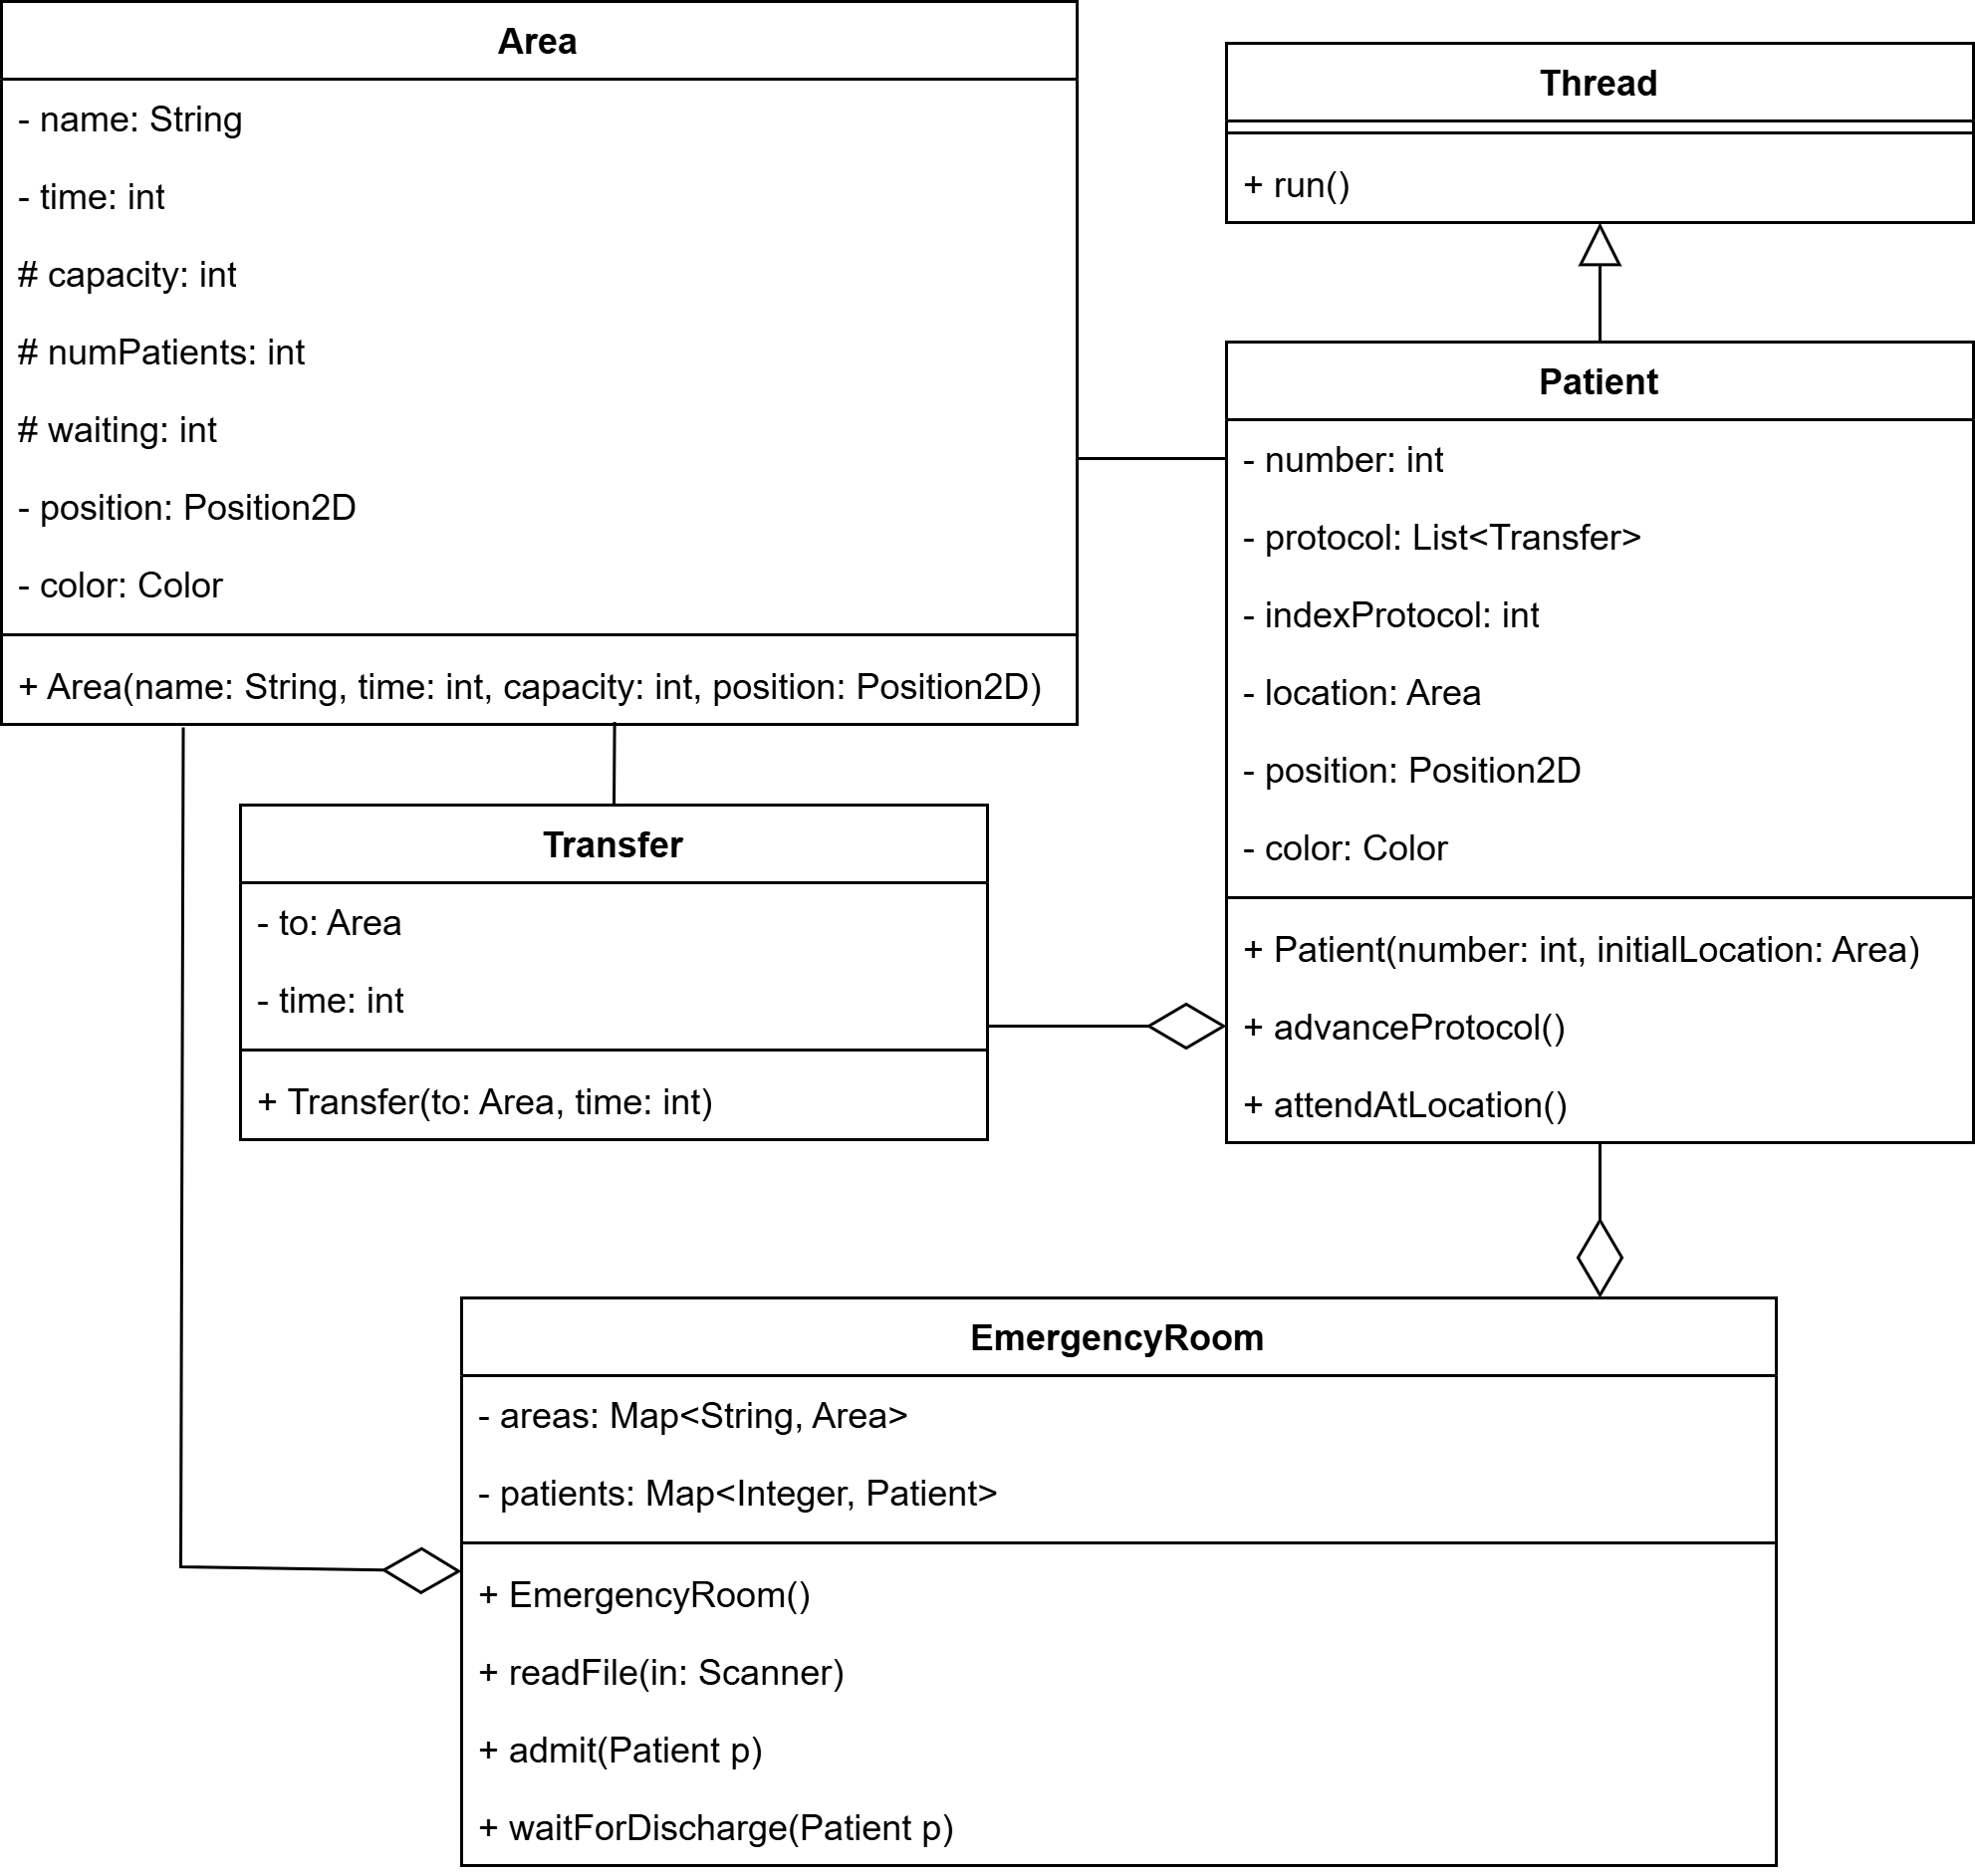
\includegraphics[width=\textwidth]{files/ALED5-DataModel.png}
  \caption{Diagrama de clases del simulador del servicio de Urgencias 2.0.}
  \label{fig:dataModel}
\end{figure}

Fíjese en que ahora \code{Area} cuenta con tres atributos nuevos:

\begin{itemize}
    \item \code{capacity}: Un \code{int} que representa el número máximo de pacientes que pueden atenderse en esa sección al mismo tiempo. Este valor se especifica en el momento de creación del \code{Area} y, como podrá observar, el constructor de la clase ha cambiado para incluir también este atributo.
    \item \code{numPatients}: Un \code{int} que indica cuántos pacientes están siendo atendidos en este momento. Este número siempre debe ser igual o inferior a \code{capacity}. Cuando se crea un \code{Area} nueva este número es 0, y nunca puede ser inferior a este valor (no se puede estar atendiendo a un número negativo de pacientes).
    \item \code{waiting}: Un \code{int} que almacena el número de pacientes que están esperando a ser atendidos en esta sección. Este número puede ser tan grande como sea necesario; es decir, que no hay límite al número de pacientes que pueden estar esperando para entrar. Cuando se crea un \code{Area} nueva este número es 0, y nunca puede ser inferior a este valor (no puede hacer un número negativo de pacientes esperando).
\end{itemize}

Observe el código de la clase \code{Area} (está en el paquete \code{es.upm.dit.aled.lab5}) que se le proporciona y fíjese bien en las partes que tendrá que implementar (las marcadas como \code{TODO}). Tenga en cuenta que, a diferencia de en prácticas anteriores, en esta tendrá que implementar los métodos por completo, incluyendo su cabecera (en lugar de únicamente el cuerpo).

\textbf{Responda a las siguientes preguntas:}

\begin{itemize}
    \item ¿Puede el atributo \code{capacity} de \code{Area} cambiar durante la ejecución del programa? Si es así, ¿en qué circunstancias?, ¿cuánto se incrementará o reducirá cada vez?
    \item ¿Puede el atributo \code{numPatients} de \code{Area} cambiar durante la ejecución del programa? Si es así, ¿en qué circunstancias?, ¿cuánto se incrementará o reducirá cada vez?
    \item ¿Puede el atributo \code{waiting} de \code{Area} cambiar durante la ejecución del programa? Si es así, ¿en qué circunstancias?, ¿cuánto se incrementará o reducirá cada vez?
\end{itemize}

\subsubsection{Monitores}

En la programación concurrente, un monitor es una clase que encapsula y protege todos los accesos (tanto lecturas como escrituras) a un recurso compartido. En lo que a esta práctica respecta, vamos a tener un monitor: la clase \code{Area}, que posee varios atributos que son susceptibles de ser modificados por varios agentes (los pacientes) al mismo tiempo. Por tanto, la clase \code{Area} deberá proteger estos atributos, asegurándose de que hay exclusión mutua en todos los fragmentos de código en los que se accede a ellos. Recuerde que estos fragmentos en los que se accede a recursos compartidos se denominan ``regiones críticas''.

Para implementar un monitor en Java, lo que se debe hacer es declarar los métodos que contengan regiones críticas como sincronizados.

\textbf{Responda a las siguientes preguntas:}

\begin{itemize}
    \item ¿Qué atributos de \code{Area} son compartidos?
    \item ¿Qué métodos de \code{Area} contienen regiones críticas?
    \item ¿Cómo se indica en Java que un método es sincronizado?
\end{itemize}

\subsubsection{Nuevo formato de archivos}
\label{sec:archivo}

Ahora abra el archivo \code{er\_data.txt}, que se encuentra en la carpeta \code{er}. Este archivo contiene la información necesaria para simular un servicio de Urgencias concreto. Aunque es muy parecido al de la práctica 4, contiene una diferencia importante. Fíjese en la información relativa a las secciones:

\begin{verbatim}
AREA  80  80 1000 2 Admision
AREA 160 320 1500 3 Triaje
AREA 160 200 3000 10 SalaEspera
AREA 320  80 3000 2 Box_Trauma
...
\end{verbatim}

Estas líneas ahora contienen un cuarto número entero, que indica cuántos pacientes puede estar atendiendo al mismo tiempo cada sección (es decir, su \code{capacity}). En este ejemplo, la sección ``Triaje'' podrá aceptar hasta a 3 pacientes al mismo tiempo.

Si observa el código del método \code{readFile(Scanner in)} de la clase \code{EmergencyRoom}, que es el que procesa estos archivos, verá que ha sido modificado respecto al de la práctica 4 para tener esto en cuenta:

\begin{minted}[
  frame=lines, % Adds a frame around the code
  framesep=2mm,
  % linenos % Enables line numbers
]{java}
...
int capacity = in.nextInt();
...
Area area = new Area(name, time, capacity, new Position2D(x, y));
...				
\end{minted}

Por lo demás, \code{EmergencyRoom} no ha experimentado ningún otro cambio. Lo mismo puede decirse de \code{Transfer} y \code{Simulation}.

\subsubsection{Nueva interfaz gráfica}

Dentro del paquete \code{es.upm.dit.aled.lab5.gui} se encuentran las clases necesarias para ejecutar una interfaz gráfica que permite visualizar el movimiento de los pacientes por el servicio de Urgencias. Respecto a la práctica 4, solo se ha modificado la clase \code{EmergencyRoomGUI}, que ahora muestra en la caja correspondiente a cada sección cuántos pacientes está atendiendo en este momento, cuántos pacientes puede atender en total, y cuántos pacientes están esperando.

La Figura \ref{fig:sampleSimulation} muestra una captura de esta interfaz gráfica en la que se puede ver que ``Box Trauma'' está atendiendo a 1 paciente cuando su capacidad total es de 2 pacientes, mientras que ``Box Criticos'' está llena (solo admite a 1 paciente) y tiene a 5 pacientes esperando.

\begin{figure}[!htbp]
  \centering
  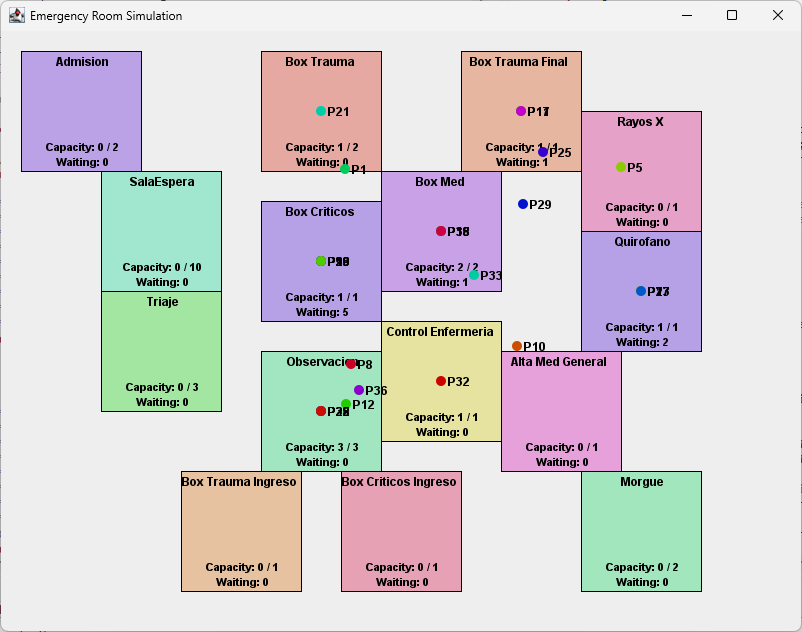
\includegraphics[width=\textwidth]{files/sampleSimulation.png}
  \caption{Simulación del servicio de Urgencias.}
  \label{fig:sampleSimulation}
\end{figure}

Pero no se preocupe, porque nada de esto le afecta. \code{EmergencyRoomGUI} sigue teniendo los mismos métodos que antes y estos se utilizan de la misma forma.

\sombreado{Patrón singleton}{Sí, \code{EmergencyRoomGUI} sigue siendo un \textit{singleton}; no se olvide de usar \code{getInstance()}.}

\subsection{Objetivo y descarga de la práctica}

El objetivo de esta práctica es mejorar el programa de simulación de un servicio de Urgencias, de manera que tenga en cuenta la capacidad de cada una de las secciones de dicho servicio. Para ello tendrá que implementar un monitor que controle el acceso a los recursos compartidos (las secciones) por parte de los agentes (los pacientes).

La práctica está disponible en GitHub, en la siguiente dirección de Internet (URI):

\href{https://github.com/rgarciacarmona/ALED-lab5}{https://github.com/rgarciacarmona/ALED-lab5}

Recuerde que, para poder importar el repositorio en Eclipse debe seleccionar \textit{File $\to$ Import...} y, de entre las opciones disponibles, \textit{Git $\to$ Projects from Git $\to$ Clone URI}. A continuación le aparecerá un menú en el que tendrá que introducir la URI que aparece en el párrafo anterior.

Una vez descargado el código de la práctica, verá que este está compuesto de dos paquetes:

\begin{itemize}
    \item \code{es.upm.dit.aled.lab5}: Que corresponde al código que simula el servicio de Urgencias.
    \item \code{es.upm.dit.aled.lab5.gui}: Que contiene las clases que permiten visualizar el movimiento de los pacientes y la ocupación de las secciones en tiempo real.
\end{itemize}

Enhorabuena, ya ha terminado con el trabajo previo a la sesión de laboratorio. Las secciones de la \ref{sec:laboratorio} en adelante puede realizarlas en clase.

\section{Control de acceso a secciones}
\label{sec:laboratorio}

Antes de seguir, asegúrese de que le queda meridianamente claro que:

\begin{itemize}
    \item Los objetos de la clase \code{Area} contienen recursos compartidos, y por tanto el código de esta clase debe encargarse de proteger su acceso. Este es el \textbf{monitor}.
    \item Los objetos de la clase \code{Patient} van a intentar utilizar los recursos compartidos, usando para ello los métodos de \code{Area}. Estos son los \textbf{agentes}.
\end{itemize}

Con esto en mente, primero implementará los métodos que faltan del monitor y, posteriormente, modificará el comportamiento de los agentes para que usen dichos métodos de la forma correcta.

\subsection{Implementación del monitor}

Si observa el código fuente de \code{Area} verá que contiene los comentarios de varios métodos que no solo no están implementados, sino tampoco definidos (no está escrita su cabecera). Su primera tarea será, en base a los comentarios antes mencionados, definir (de nuevo, escribir las cabeceras) de los métodos siguientes:

\begin{itemize}
    \item \code{getCapacity}: Devuelve el valor actual de \code{capacity}.
    \item \code{getNumPatients}: Devuelve el valor actual de \code{numPatients}.
    \item \code{getWaiting}: Devuelve el valor actual de \code{waiting}.
    \item \code{enter}: Un \code{Patient} que esté intentando entrar en esta \code{Area} para ser atendido llamará a este método.
    \item \code{exit}: Un \code{Patient} que ya haya sido atendido llamará a este método antes de avanzar al siguiente \code{Transfer} de su protocolo.
\end{itemize}

Los comentarios le indican qué parámetros y qué tipos de retorno deben tener los métodos, si es que no los ha deducido usted mismo.

\textbf{Importante:} Asegúrese de que los métodos que vayan a contener regiones críticas estén sincronizados.

\sombreado{Sincronización también para lectura}{No se olvide de que el código que accede a un recurso compartido solo para leerlo (sin modificarlo) también es una sección crítica. Esto se debe a que, aunque la hebra que lee el recurso no lo modifique ella misma (no puede haber colisión de escrituras), eso no quiere decir que dicho recurso no esté siendo modificado al mismo tiempo por otro agente distinto (sí puede haber colisión de escritura-lectura).}

A continuación, termine de implementar el constructor de \code{Area}, pues solo contiene el código en el que se le asigna el \code{color} por defecto.

Ahora implemente los métodos que definió antes. \code{getCapacity}, \code{getNumPatients} y \code{getWaiting} no tienen más misterio, pues son accesores normales y corrientes, pero los métodos \code{enter} y \code{exit} requieren de algo más de reflexión.

\subsubsection{Método \code{enter}}

Cuando un \code{Patient} llama a este método, eso quiere decir que está intentando acceder a un recurso compartido. Esto solo será posible si ahora mismo el número de pacientes que están siendo atendidos en esa sección es inferior a la capacidad de la misma. Por tanto, el método \code{enter} deberá contener un bucle \code{while} que compruebe esta condición y, de no cumplirse, haga a la hebra del paciente esperar mediante una llamada a \code{wait()}.

Además, \code{enter} también deberá encargarse de modificar los atributos \code{numPatients} y \code{waiting}. Intente pensar usted mismo cuánto deberían incrementarse y/o decrementarse y en qué momento. Si no consigue apañarse, un poco más abajo tiene la solución.

\vspace{1cm}

...

\vspace{1cm}

¿Seguro que no se le ocurre? Piense un poco más...

\vspace{1cm}

Venga, se lo cuento, pero solo para que compruebe que la solución que se le había ocurrido a usted es la correcta. Estos dos atributos deberán modificarse de la siguiente forma:
\begin{itemize}
    \item Si un paciente se ve forzado a esperar porque la sección ya está llena, \code{waiting} deberá incrementarse en 1.
    \item Si un paciente logra acceder a la sección, \code{numPatients} deberá incrementarse en 1.
    \item Si un paciente que estaba esperando logra acceder a la sección, \code{numWaiting} deberá reducirse en 1.
\end{itemize}

\sombreado{El bucle while}{Es \textbf{muy importante} que la comprobación de la condición de acceso a la sección se haga dentro de un bucle \code{while}, y no solo una única vez. La razón es que, incluso aunque una hebra se haya despertado tras un \code{wait()}, eso no asegura que la condición se cumpla ahora; otra hebra podría haber modificado el recurso compartido en el tiempo que pasa desde que se despierta a la hebra hasta que esta se ejecuta. O puede incluso que la hebra haya sido despertada por una razón distinta a que la condición que la hizo esperar se cumpla.}

\subsubsection{Método \code{exit}}

Este método deberá indicar que se ha liberado una plaza en el \code{Area} (modificando \code{numPatients}) y despertar a todas las hebras de los \code{Patients} que estaban esperando para acceder. Esto último puede hacerse mediante una llamada al método \code{notifyAll()}.

\sombreado{¡Pero si no necesito al paciente!}{Es posible que al implementar los métodos \code{enter} y \code{exit} se haya dado cuenta de que, a pesar de que ambos tienen como parámetro un objeto \code{Patient}, luego este no necesitan usarlo para nada. La razón de esto es que tener la referencia al paciente que está intentando entrar o salir de la sección en estos métodos es muy útil, ya que puede usarse para imprimir por pantalla mensajes de información que indiquen en qué estado se encuentra cada \code{Patient} (esperando para entrar, siendo atendido, saliendo...).

Además, en la sección \ref{sec:listaOrdenada} verá que sí que necesita al paciente para el método \code{enter}.}

\subsection{Modificación de \code{Patient}}

Ahora que ha terminado de implementar el monitor, es necesario que modifique el comportamiento de \code{Patient} (su método \code{run()}) para que haga uso de los métodos \code{enter} y \code{exit} que acaba de escribir. Los pasos que debe seguir cada paciente ahora son:

\begin{enumerate}
    \item Intentar acceder a la ubicación actual (\code{enter}).
    \item Ser atendido en la ubicación actual.
    \item Salir de la ubicación actual (\code{exit}).
    \item Avanzar al siguiente paso en su protocolo.
    \item Volver al paso 1.
\end{enumerate}

Para los detalles sobre los puntos 2, 4 y 5, consulte la práctica 4. Idealmente, no debería necesitar programarlos, pues ya escribió en dicha práctica el código que hacía esto.

\subsection{Ejecución de la simulación}
\label{sec:ejecucion}

Pues ya estaría. Solo le queda ejecutar el método \code{main()} de la clase \code{Simulation}. No se olvide de crear una configuración de lanzamiento que pase como primer argumento la ubicación del archivo de texto que contiene los datos del servicio de Urgencias: \code{er\_data.txt}, que se encuenta en la carpeta \code{er}. Si todo va bien, debería ver como los pacientes esperan pacientemente (jeje) a ser atendidos, como en la Figura \ref{fig:sampleSimulation}.

\section{Control de acceso con lista ordenada}
\label{sec:listaOrdenada}

Su servicio de Urgencias tiene un problema: no se atiende a los pacientes en orden de llegada. Cuando un \code{Patient} sale de un \code{Area}, despierta a todos los que estaban esperando (mediante \code{notifyAll()}). En ese momento se produce una suerte de ``estampida virtual'', en la que todos los pacientes intentan entrar corriendo en la sección, algo que solo conseguirá el que sea más rápido (o tenga más suerte). Esto podría desembocar en situaciones que en programación concurrente se llaman de ``inanición'', en las que un \code{Patient} nunca logra entrar en un \code{Area} porque continúan llegando pacientes nuevos que se le ``cuelan''

\subsection{Clase \code{AreaQueue}}

Para evitar esto va a implementar un versión mejorada de \code{Area}, llamada \code{AreaQueue}, que utiliza una cola para respetar el orden de llegada de los pacientes. La Figura \ref{fig:dataModelQueue} le muestra lo que necesita saber de esta clase para poder implementarla. Como puede observar, esta nueva clase extiende a \code{Area}, por lo que hereda todos los métodos y atributos de esta. Eso incluye los métodos que usted mismo programó en la sección \ref{sec:laboratorio}. Solo añade un constructor y reimplementa (sobreescribe usando \code{@Override}) el método \code{enter} de su clase madre.

\begin{figure}[!htbp]
  \centering
  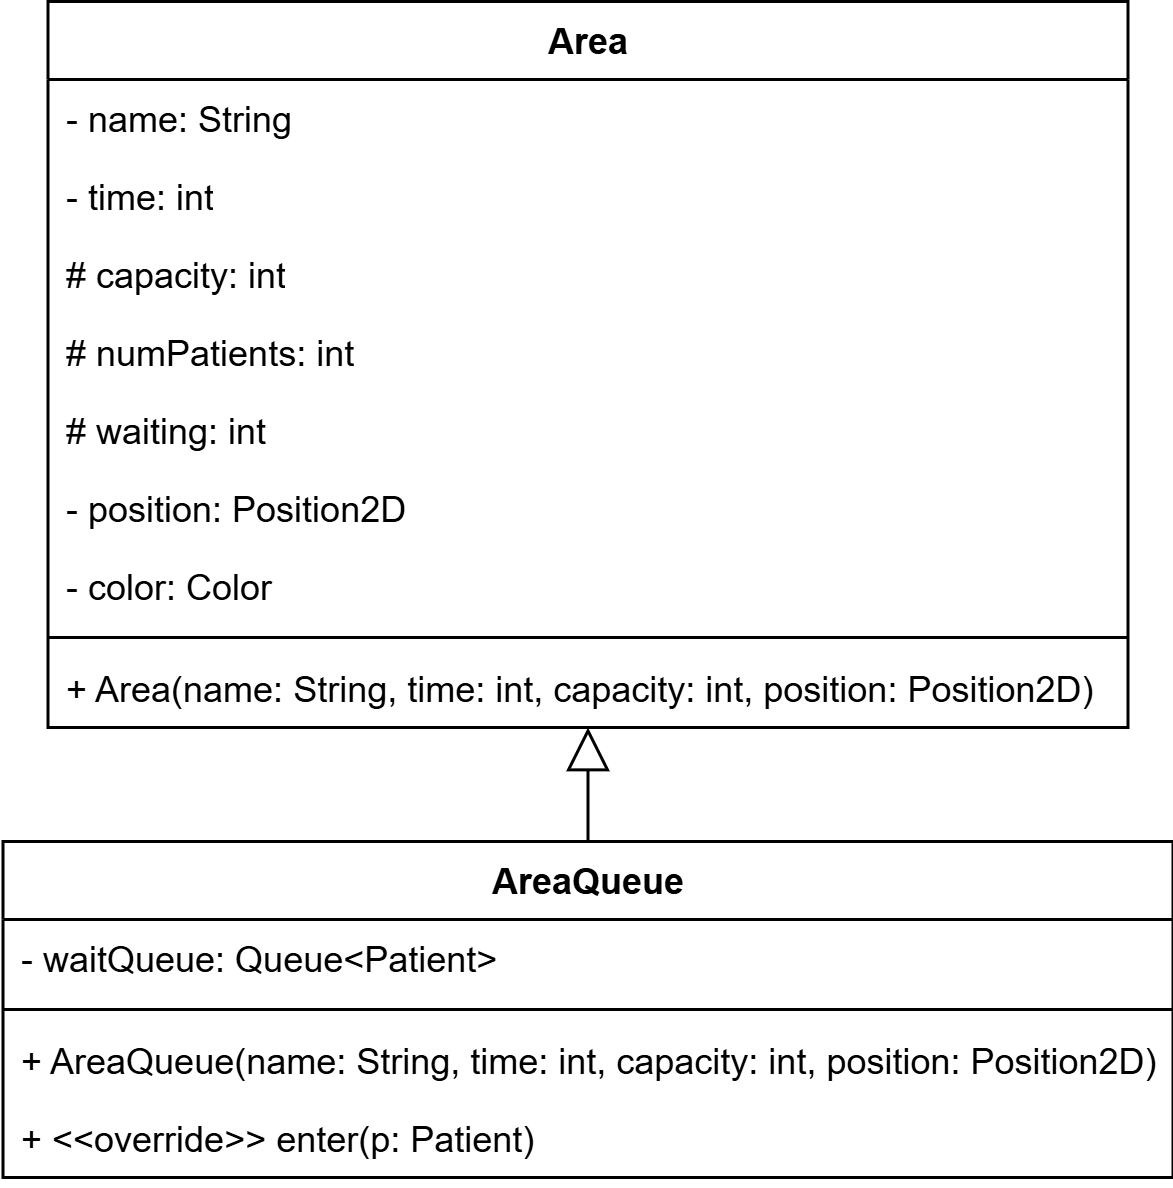
\includegraphics[width=0.5\textwidth]{files/ALED5-DataModelQueue.png}
  \caption{Diagrama de clases de \code{AreaQueue}.}
  \label{fig:dataModelQueue}
\end{figure}



En esta sección implementará por completo esta clase. Sí, desde cero; esta vez no se le proporciona un esqueleto que tendrá que rellenar. A estas alturas del curso ya es usted un programador hecho y derecho, por lo que no tendrá ningún problema. Además, esta tarea no es tan laboriosa como en un principio podría parecer, ya que al ser \code{AreaQueue} hija de la clase \code{Area}, la mayor parte del código de la clase ya está implementado (se hereda de \code{Area}). De hecho, fíjese otra vez en la Figura \ref{fig:dataModelQueue}; verá que en en la clase \code{AreaQueue} solo aparecen indicados dos métodos y un atributo. Estas tres cosas es lo que tiene que implementar.

\sombreado{Protected}{Quizá haya observado que en la clase \code{Area} hay tres atributos que no son \code{private}, sino \code{protected}: \code{capacity}, \code{numPatients} y \code{waiting}. Si revisa sus apuntes de Fundamentos de Programación verá que \code{protected} es un tipo de visibilidad que se usa precisamente en situaciones como esta, en las que queremos que las clases hijas (o en el mismo paquete) puedan acceder a los atributos, pero que estos sigan siendo privados para clases que se encuentren en otros paquetes.}

Fíjese en que el método \code{enter}, aunque ya estaba presente en la clase \code{Area}, ahora vuelve a aparecer en \code{AreaQueue}, pero precedido del texto \code{<<override>>}. Este texto indica que la clase tiene que reimplementar un método que ya poseía la clase madre, pues la funcionalidad ha cambiado. Y es que ahora ya no es suficiente con comprobar que se cumple la condición de ocupación (que \code{numPatients} sea menor que \code{capacity}), sino que también es necesario que el paciente que quiere entrar sea \textbf{el primero de la cola de espera}. Esta cola de espera está representada por el atributo \code{waitQueue}.

A la hora de implementar \code{AreaQueue}, tenga en cuenta los siguientes consejos:

\begin{itemize}
    \item \code{Queue} no es una clase, sino un interfaz. Por tanto, no puede crear directamente objetos de \code{Queue}, sino que tendrá que usar su implementación: \code{LinkedList}.
    \item Tendrá que utilizar los siguientes métodos del interfaz \code{Queue}:
    \begin{itemize}
        \item \code{add(Patient p)}: Añade a \code{p} al \textbf{final} de la cola.
        \item \code{remove():} Devuelve el \code{Patient} que se encuentra al \textbf{principio} de la cola y lo elimina, de tal forma que el siguiente elemento de la cola pasa a ser el primero.
        \item \code{peek()}: Devuelve el \code{Patient} que se encuentra al \textbf{principio} de la cola. La diferencia con \code{remove()} es que \code{peek()} no elimina (saca) al elemento de la cola, simplemente permite ver cuál es.
    \end{itemize}
    \item Para indicar que el método \code{enter} reimplementa el de la clase madre, tendrá que usar la anotación Java \code{@Override}:
\begin{minted}[
  frame=lines, % Adds a frame around the code
  framesep=2mm,
  % linenos % Enables line numbers
]{java}
@Override
public synchronized void enter(Patient patient) {
...
}
\end{minted}
\end{itemize}

\subsection{Ejecución de la simulación}

Ya solo queda ejecutar la simulación. Pero, para esto, antes debe modificar una línea de la clase \code{EmergencyRoom} para que utilice la clase \code{AreaQueue} que acaba de crear, en lugar de \code{Area}. Sustituya el código que se encuentra en la línea 97 de \code{EmergencyRoom} por el siguiente:

\begin{minted}[
  frame=lines, % Adds a frame around the code
  framesep=2mm,
  % linenos % Enables line numbers
]{java}
Area area = new AreaQueue(name, time, capacity, new Position2D(x, y));
\end{minted}

Por último, ejecute de nuevo la simulación de la sección \ref{sec:ejecucion}. Si todo ha ido bien, verá como los pacientes son atendidos en orden de llegada a cada zona del servicio de Urgencias.

Enhorabuena. Ha terminado la práctica.

\section{Extras} 

Si siente curiosidad, pruebe a llevar a cabo las siguientes modificaciones del proyecto. ¡Ojo!, las dos últimas implican un trabajo de desarrollo considerable.

\begin{itemize}
    \item Modifique el código para que tanto el tiempo de atención de un \code{Area} como el tiempo de traslado de un \code{Transfer} sean tiempos medios. El tiempo real se calculará de forma aleatoria, estando comprendido entre \code{time-1000} milisegundos y \code{time+1000} milisegundos.
    \item Añada al proyecto un nuevo agente: el \code{Doctor}. \code{Doctor} estará asignado a un conjunto de \code{Areas} e irá atendiendo a los pacientes que acudan a dichas secciones. Si realiza esta modificación, las \code{Area} ya no tendrán \code{capacity} ni \code{numPatients}, pues cuántos pacientes estén siendo atendidos dependerá de qué \code{Doctors} están en dicha \code{Area}. De hecho, ya no son las \code{Areas} las que ``atienden'', sino los \code{Doctors}.
    \item Modifique el proyecto para que, cuando un paciente tiene que esperar, vaya al \code{Area} cuyo nombre sea ``SalaEspera''. Si un \code{Patient} tiene que entrar en ``SalaEspera'' y esta está llena, en lugar de eso abandonará el hospital (o, si lo prefiere, morirá, que es más dramático). Asuma que el tiempo necesario para trasladarse a ``SalaEspera`` cuando este traslado no es parte del protocolo (un \code{Transfer}) es siempre de 1000 milisegundos.
\end{itemize}

\end{document}